\documentclass[border=4pt]{standalone}
\usepackage{times}
\usepackage{tikz}
\usepackage{amsmath}
\usepackage{amssymb}
\usetikzlibrary{arrows.meta,positioning,backgrounds,fit,calc,shapes.geometric}
\DeclareMathSizes{8}{10}{7}{5}

% ---- palette ----
\definecolor{stagefill}{HTML}{F4F6FB}
\definecolor{stageline}{HTML}{C7CFE0}
\definecolor{ink}{HTML}{1F2733}
\definecolor{flow}{HTML}{5B6B86}
\definecolor{rootc}{HTML}{2B2F3A}
\definecolor{bannerfill}{HTML}{EAEEF7}
\definecolor{bannerline}{HTML}{B7C2D8}
\definecolor{estc}{HTML}{3F7CAC}
\definecolor{truthc}{HTML}{2B2F3A}
\definecolor{nullc}{HTML}{B9C0CE}
\definecolor{okc}{HTML}{4FA06B}
% frontier family colors
\definecolor{fClaude}{HTML}{C7693C}
\definecolor{fGPT}{HTML}{4FA06B}
\definecolor{fGemini}{HTML}{3F7CAC}
\definecolor{fOpen}{HTML}{8A6FB0}
\definecolor{fDeepSeek}{HTML}{2A9D8F}

\begin{document}
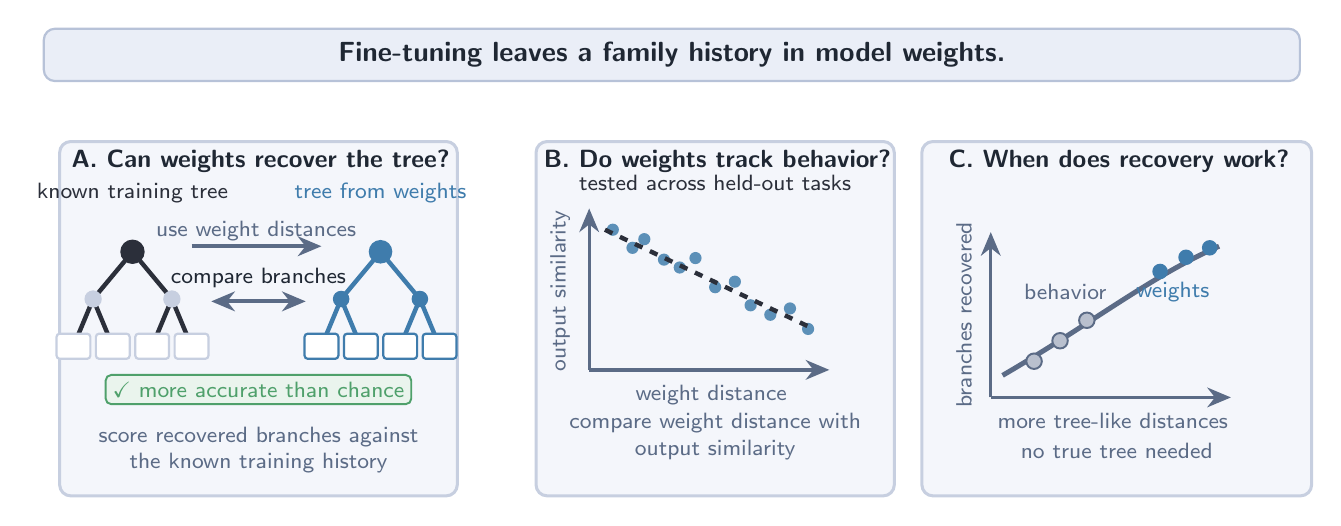
\begin{tikzpicture}[
  font=\sffamily,
  >={Stealth[length=3.0mm,width=2.5mm]},
  panel/.style={draw=stageline,line width=1.1pt,rounded corners=4pt,fill=stagefill},
  ptitle/.style={font=\sffamily\small\bfseries,text=ink},
  scap/.style={font=\sffamily\footnotesize,text=flow,align=center},
  mdl/.style={draw=stageline,fill=white,rounded corners=1.2pt,minimum width=4.3mm,minimum height=3.2mm,line width=0.8pt,inner sep=0pt},
  flowarrow/.style={->,line width=1.7pt,draw=flow},
]

% ===================== TOP CLAIM BANNER =====================
\node[draw=bannerline,fill=bannerfill,rounded corners=4pt,line width=0.8pt,
      text width=15.6cm,align=center,inner sep=5pt,
      font=\sffamily\normalsize\bfseries,text=ink] (banner) at (7.9,5.55)
  {Fine-tuning leaves a family history in model weights.};

% ===================== PANEL A: controlled whitebox =====================
\begin{scope}
  \node[panel,minimum width=5.05cm,minimum height=4.5cm] (PA) at (2.65,2.2){};
  \node[ptitle,anchor=north] at (PA.north) {\,A.\ Can weights recover the tree?};

  % true tree (left)
  \node[font=\sffamily\footnotesize,text=truthc] at (1.05,3.80) {known training tree};
  \coordinate (tr) at (1.05,3.05);
  \coordinate (ta) at (0.55,2.45); \coordinate (tb) at (1.55,2.45);
  \coordinate (ta1) at (0.30,1.85);\coordinate (ta2) at (0.80,1.85);
  \coordinate (tb1) at (1.30,1.85);\coordinate (tb2) at (1.80,1.85);
  \draw[truthc,line width=1.6pt] (tr)--(ta) (tr)--(tb) (ta)--(ta1) (ta)--(ta2) (tb)--(tb1) (tb)--(tb2);
  \node[circle,fill=rootc,inner sep=0pt,minimum size=3.1mm] at (tr){};
  \foreach \p in {ta,tb}{\node[circle,fill=stageline,inner sep=0pt,minimum size=2.2mm] at (\p){};}
  \foreach \p in {ta1,ta2,tb1,tb2}{\node[mdl] at (\p){};}

  % recovered tree (right)
  \node[font=\sffamily\footnotesize,text=estc] at (4.20,3.80) {tree from weights};
  \coordinate (er) at (4.20,3.05);
  \coordinate (ea) at (3.70,2.45); \coordinate (eb) at (4.70,2.45);
  \coordinate (ea1) at (3.45,1.85);\coordinate (ea2) at (3.95,1.85);
  \coordinate (eb1) at (4.45,1.85);\coordinate (eb2) at (4.95,1.85);
  \draw[estc,line width=1.6pt] (er)--(ea) (er)--(eb) (ea)--(ea1) (ea)--(ea2) (eb)--(eb1) (eb)--(eb2);
  \node[circle,fill=estc,inner sep=0pt,minimum size=3.0mm] at (er){};
  \foreach \p in {ea,eb}{\node[circle,fill=estc,inner sep=0pt,minimum size=2.1mm] at (\p){};}
  \foreach \p in {ea1,ea2,eb1,eb2}{\node[mdl,draw=estc] at (\p){};}

  % Build a tree from model-weight distances, then compare its branches with truth.
  \draw[->,line width=1.4pt,draw=flow] (1.80,3.12)--(3.45,3.12);
  \node[font=\sffamily\footnotesize,text=flow] at (2.62,3.32) {use weight distances};
  \draw[<->,line width=1.4pt,draw=flow] (2.05,2.42)--(3.25,2.42);
  \node[font=\sffamily\footnotesize,text=ink] at (2.65,2.72) {compare branches};
  \node[draw=okc,rounded corners=2pt,line width=0.7pt,fill=okc!12,
        font=\sffamily\footnotesize,text=okc,inner sep=2.5pt] at (2.65,1.30)
        {$\checkmark$ more accurate than chance};
  \node[scap,anchor=north] at (2.65,0.95) {score recovered branches against\\the known training history};
\end{scope}

% ===================== PANEL B: weights -> behavior =====================
\begin{scope}
  \node[panel,minimum width=4.55cm,minimum height=4.5cm] (PB) at (8.45,2.2){};
  \node[ptitle,anchor=north] at (PB.north) {\,B.\ Do weights track behavior?};
  \node[font=\sffamily\footnotesize,text=truthc] at (8.45,3.92) {tested across held-out tasks};

  % scatter axes
  \begin{scope}[shift={(6.85,1.55)}]
    \draw[->,line width=1.2pt,draw=flow] (0,0)--(3.05,0);
    \draw[->,line width=1.2pt,draw=flow] (0,0)--(0,2.05);
    \node[font=\sffamily\footnotesize,text=flow,anchor=north] at (1.55,-0.07) {weight distance};
    \node[font=\sffamily\footnotesize,text=flow,rotate=90,anchor=south] at (-0.12,1.0) {output similarity};
    % points (negative trend)
    \foreach \x/\y in {0.30/1.78,0.55/1.55,0.70/1.66,0.95/1.40,1.15/1.30,1.35/1.42,1.60/1.05,1.85/1.12,2.05/0.82,2.30/0.70,2.55/0.78,2.78/0.52}{
      \fill[estc!85!white] (\x,\y) circle (2.2pt);
    }
    \draw[truthc,line width=1.6pt,dashed] (0.20,1.78)--(2.85,0.52);
  \end{scope}
  \node[scap,anchor=north] at (8.45,1.12) {compare weight distance with\\output similarity};
\end{scope}

% ===================== PANEL C: label-free additivity flags trust, weights AND behavior =====================
\begin{scope}
  \node[panel,minimum width=4.95cm,minimum height=4.5cm] (PC) at (13.55,2.2){};
  \node[ptitle,anchor=north] at (PC.north) {\,C.\ When does recovery work?};

  \begin{scope}[shift={(11.95,1.20)}]
    % axes
    \draw[->,line width=1.2pt,draw=flow] (0,0)--(3.05,0);
    \draw[->,line width=1.2pt,draw=flow] (0,0)--(0,2.10);
    \node[font=\sffamily\footnotesize,text=flow,anchor=north] at (1.55,-0.07) {more tree-like distances};
    \node[font=\sffamily\footnotesize,text=flow,rotate=90,anchor=south] at (-0.12,1.05) {branches recovered};
    % single label-free A -> recovery trend; BOTH modalities land on it
    \draw[flow,line width=1.8pt] (0.15,0.28) .. controls (1.30,0.95) and (2.05,1.55) .. (2.90,1.92);
    % behavior points (lower A, still on the curve)
    \foreach \x/\y in {0.55/0.46,0.88/0.72,1.22/0.98}{
      \fill[nullc] (\x,\y) circle (2.8pt); \draw[flow,line width=0.7pt] (\x,\y) circle (2.8pt);}
    % weight points (high A, high recovery, on the same curve)
    \foreach \x/\y in {2.15/1.60,2.48/1.78,2.78/1.90}{\fill[estc] (\x,\y) circle (2.8pt);}
    \node[font=\sffamily\footnotesize,text=flow,anchor=west] at (0.30,1.34) {behavior};
    \node[font=\sffamily\footnotesize,text=estc,anchor=east] at (2.90,1.34) {weights};
  \end{scope}
  \node[scap,anchor=north] at (13.55,0.74) {no true tree needed};
\end{scope}

\end{tikzpicture}
\end{document}
